\chapter{Synthetic Lethal Analysis of Gene Expression Data}
\label{chap:SLIPT}

%\section{Aims and Significance}

\paragraph{Aims}

  \begin{itemize}
   \item Pathway Structure of Candidate Synthetic Lethal Genes for \textit{\textit{CDH1}} from TCGA breast data
   
   \bigskip
   
   \item Comparisons to Experimental siRNA Screen Candidates
   
   \bigskip
   
   \item Replication of Pathways across in TCGA Stomach data
  \end{itemize}

\paragraph{Summary}

    
  \begin{itemize}
   \item We have developed a Synthetic Lethal detection method that generates a high number of synthetic lethal candidates
   
   \bigskip
   
   \item Pathways in cell signalling, extracellular matrix, and cytoskeletal functions were supported with experimental candidates and the known functions of E-cadherin
   
   \bigskip
   
   \item Several candidate pathways were supported by mutation analysis and replicated across breast and stomach cancer
   
   \bigskip
   
   \item Translation and immune functions were uniquely detected by the computational approach which may be explained by differences between patient samples and cell line models
   
   \bigskip
   
   \item There remains the need to identify actionable genes within these pathways, relationships with experimental candidates, and how these pathways may affect viability when lost
  \end{itemize}

\section{Synthetic lethal genes in breast cancer}

\begin{itemize}
 \item exprSL
 \item mtSL
 \item heatmap
\end{itemize}


\begin{table*}[!ht]
\caption{Candidate synthetic lethal genes against E-cadherin from SLIPT}
\label{tab:gene_SL}
\resizebox{\textwidth}{!}{
\begin{tabular}{>{\em}sl^c^c^c^l^l}
\rowstyle{\bfseries}
 \em{Gene} & Observed Low-Low & Expected Low-Low & $\chi^2$ value & raw p-val & p-val (FDR) \\ 
  \hline
  \rowcolor{black!10}
TRIP10 & 62 & 130 & 162 & $5.65 \times 10^{-34}$ & $1.84 \times 10^{-31}$ \\
  \rowcolor{black!5} 
  EEF1B2 & 56 & 130 & 158 & $3.10 \times 10^{-33}$ & $9.45 \times 10^{-31}$ \\
  \rowcolor{black!10} 
  GBGT1 & 61 & 131 & 156 & $1.08 \times 10^{-32}$ & $3.14 \times 10^{-30}$ \\
  \rowcolor{black!5} 
  ELN & 81 & 130 & 149 & $3.46 \times 10^{-31}$ & $8.82 \times 10^{-29}$ \\
  \rowcolor{black!10} 
  TSPAN4 & 78 & 130 & 146 & $1.63 \times 10^{-30}$ & $3.79 \times 10^{-28}$ \\
  \rowcolor{black!5} 
  GLIPR2 & 72 & 130 & 146 & $1.68 \times 10^{-30}$ & $3.86 \times 10^{-28}$ \\
  \rowcolor{black!10} 
  RPS20 & 73 & 131 & 145 & $1.89 \times 10^{-30}$ & $4.28 \times 10^{-28}$ \\
  \rowcolor{black!5} 
  RPS27A & 80 & 130 & 143 & $5.53 \times 10^{-30}$ & $1.18 \times 10^{-27}$ \\
  \rowcolor{black!10} 
  EEF1A1P9 & 63 & 130 & 141 & $1.91 \times 10^{-29}$ & $3.74 \times 10^{-27}$ \\
  \rowcolor{black!5} 
  C1R & 73 & 130 & 141 & $2.05 \times 10^{-29}$ & $3.97 \times 10^{-27}$ \\
  \rowcolor{black!10} 
  LYL1 & 73 & 130 & 140 & $2.99 \times 10^{-29}$ & $5.74 \times 10^{-27}$ \\
  \rowcolor{black!5} 
  RPLP2 & 71 & 130 & 139 & $4.88 \times 10^{-29}$ & $9.07 \times 10^{-27}$ \\
  \rowcolor{black!10} 
  C10orf10 & 73 & 130 & 138 & $6.72 \times 10^{-29}$ & $1.20 \times 10^{-26}$ \\
  \rowcolor{black!5} 
  DULLARD & 74 & 131 & 138 & $9.29 \times 10^{-29}$ & $1.61 \times 10^{-26}$ \\
  \rowcolor{black!10} 
  PPM1F & 64 & 130 & 136 & $1.61 \times 10^{-28}$ & $2.65 \times 10^{-26}$ \\
  \rowcolor{black!5} 
  OBFC2A & 69 & 130 & 136 & $2.49 \times 10^{-28}$ & $3.93 \times 10^{-26}$ \\
  \rowcolor{black!10} 
  RPL11 & 70 & 130 & 136 & $2.56 \times 10^{-28}$ & $3.97 \times 10^{-26}$ \\
  \rowcolor{black!5} 
  RPL18A & 70 & 130 & 135 & $3.08 \times 10^{-28}$ & $4.70 \times 10^{-26}$ \\
  \rowcolor{black!10} 
  MFNG & 76 & 131 & 133 & $7.73 \times 10^{-28}$ & $1.12 \times 10^{-25}$ \\
  \rowcolor{black!5} 
  RPS17 & 77 & 131 & 133 & $8.94 \times 10^{-28}$ & $1.29 \times 10^{-25}$ \\
  \rowcolor{black!10} 
  MGAT1 & 73 & 130 & 132 & $1.44 \times 10^{-27}$ & $2.03 \times 10^{-25}$ \\
  \rowcolor{black!5} 
  RPS12 & 72 & 130 & 128 & $8.57 \times 10^{-27}$ & $1.12 \times 10^{-24}$ \\
  \rowcolor{black!10} 
  C10orf54 & 73 & 130 & 127 & $1.37 \times 10^{-26}$ & $1.75 \times 10^{-24}$ \\
  \rowcolor{black!5} 
  LOC286367 & 72 & 130 & 126 & $2.20 \times 10^{-26}$ & $2.70 \times 10^{-24}$ \\
  \rowcolor{black!10} 
  GMFG & 70 & 130 & 126 & $2.20 \times 10^{-26}$ & $2.70 \times 10^{-24}$ \\ 
  \hline
\end{tabular}
}
\end{table*}

\begin{table*}[!ht]
\caption{Candidate synthetic lethal genes against E-cadherin from mtSLIPT}
\label{tab:gene_mtSL}
\resizebox{\textwidth}{!}{
\begin{tabular}{>{\em}sl^c^c^c^l^l}
\rowstyle{\bfseries}
 \em{Gene} & Observed Low-Low & Expected Low-Low & $\chi^2$ value & raw p-val & p-val (FDR) \\ 
  \hline
  \rowcolor{black!10}
TFAP2B & 8 & 36.7 & 89.5 & $3.6 \times 10^{-20}$ & $8.37 \times 10^{-17}$ \\
  \rowcolor{black!5}
  ZNF423 & 15 & 36.7 & 78.8 & $7.89 \times 10^{-18}$ & $1.22 \times 10^{-14}$ \\ 
  \rowcolor{black!10}
  CALCOCO1 & 11 & 36.7 & 76.8 & $2.09 \times 10^{-17}$ & $2.59 \times 10^{-14}$ \\ 
  \rowcolor{black!5}
  RBM5 & 13 & 36.7 & 75.7 & $3.65 \times 10^{-17}$ & $4.00 \times 10^{-14}$ \\ 
  \rowcolor{black!10}
  BTG2 & 7 & 36.7 & 71.7 & $2.72 \times 10^{-16}$ & $1.81 \times 10^{-13}$ \\ 
  \rowcolor{black!5}
  RXRA & 6 & 36.7 & 70.5 & $5.00 \times 10^{-16}$ & $2.97 \times 10^{-13}$ \\ 
  \rowcolor{black!10}
  SLC27A1 & 11 & 36.7 & 70.3 & $5.42 \times 10^{-16}$ & $2.97 \times 10^{-13}$ \\ 
  \rowcolor{black!5}
  MEF2D & 12 & 36.7 & 69.6 & $7.86 \times 10^{-16}$ & $3.95 \times 10^{-13}$ \\ 
  \rowcolor{black!10}
  NISCH & 12 & 36.7 & 69.6 & $7.86 \times 10^{-16}$ & $3.95 \times 10^{-13}$ \\ 
  \rowcolor{black!5}
  AVPR2 & 9 & 36.7 & 69.2 & $9.36 \times 10^{-16}$ & $4.58 \times 10^{-13}$ \\ 
  \rowcolor{black!10}
  CRY2 & 13 & 36.7 & 68.9 & $1.07 \times 10^{-15}$ & $4.98 \times 10^{-13}$ \\ 
  \rowcolor{black!5}
  RAPGEF3 & 13 & 36.7 & 68.9 & $1.07 \times 10^{-15}$ & $4.98 \times 10^{-13}$ \\ 
  \rowcolor{black!10}
  NRIP2 & 10 & 36.7 & 68.2 & $1.58 \times 10^{-15}$ & $7.18 \times 10^{-13}$ \\ 
  \rowcolor{black!5}
  DARC & 12 & 36.7 & 66.4 & $3.76 \times 10^{-15}$ & $1.54 \times 10^{-12}$ \\ 
  \rowcolor{black!10}
  SFRS5 & 12 & 36.7 & 66.4 & $3.76 \times 10^{-15}$ & $1.54 \times 10^{-12}$ \\ 
  \rowcolor{black!5}
  NOSTRIN & 5 & 36.7 & 65.1 & $7.40 \times 10^{-15}$ & $2.70 \times 10^{-12}$ \\ 
  \rowcolor{black!10}
  KIF13B & 12 & 36.7 & 63.4 & $1.69 \times 10^{-14}$ & $5.16 \times 10^{-12}$ \\ 
  \rowcolor{black!5}
  TENC1 & 10 & 36.7 & 62.5 & $2.67 \times 10^{-14}$ & $7.40 \times 10^{-12}$ \\ 
  \rowcolor{black!10}
  MFAP4 & 12 & 36.7 & 60.5 & $7.17 \times 10^{-14}$ & $1.67 \times 10^{-11}$ \\ 
  \rowcolor{black!5}
  ELN & 13 & 36.7 & 59.7 & $1.07 \times 10^{-13}$ & $2.32 \times 10^{-11}$ \\ 
  \rowcolor{black!10}
  SGK223 & 14 & 36.7 & 59 & $1.51 \times 10^{-13}$ & $3.05 \times 10^{-11}$ \\ 
  \rowcolor{black!5}
  KIF12 & 11 & 36.7 & 58.8 & $1.74 \times 10^{-13}$ & $3.34 \times 10^{-11}$ \\ 
  \rowcolor{black!10}
  SELP & 11 & 36.7 & 58.8 & $1.74 \times 10^{-13}$ & $3.34 \times 10^{-11}$ \\ 
  \rowcolor{black!5}
  CIRBP & 9 & 36.7 & 58.7 & $1.83 \times 10^{-13}$ & $3.41 \times 10^{-11}$ \\ 
  \rowcolor{black!10}
  CTDSP1 & 9 & 36.7 & 58.7 & $1.83 \times 10^{-13}$ & $3.41 \times 10^{-11}$ \\ 
  \rowcolor{black!5}
   \hline
\end{tabular}
}
\end{table*}




\subsection{Synthetic lethal pathways in breast cancer}

Table 5.  Gene set enrichment results for subgroups of \textit{CDH1} SL partners shows functional variation.

\subsection{Expression profiles of synthetic lethal partners}

\begin{figure*}[!ht]
\begin{mdframed}
  \centering
  \resizebox{0.99 \textwidth}{!}{
    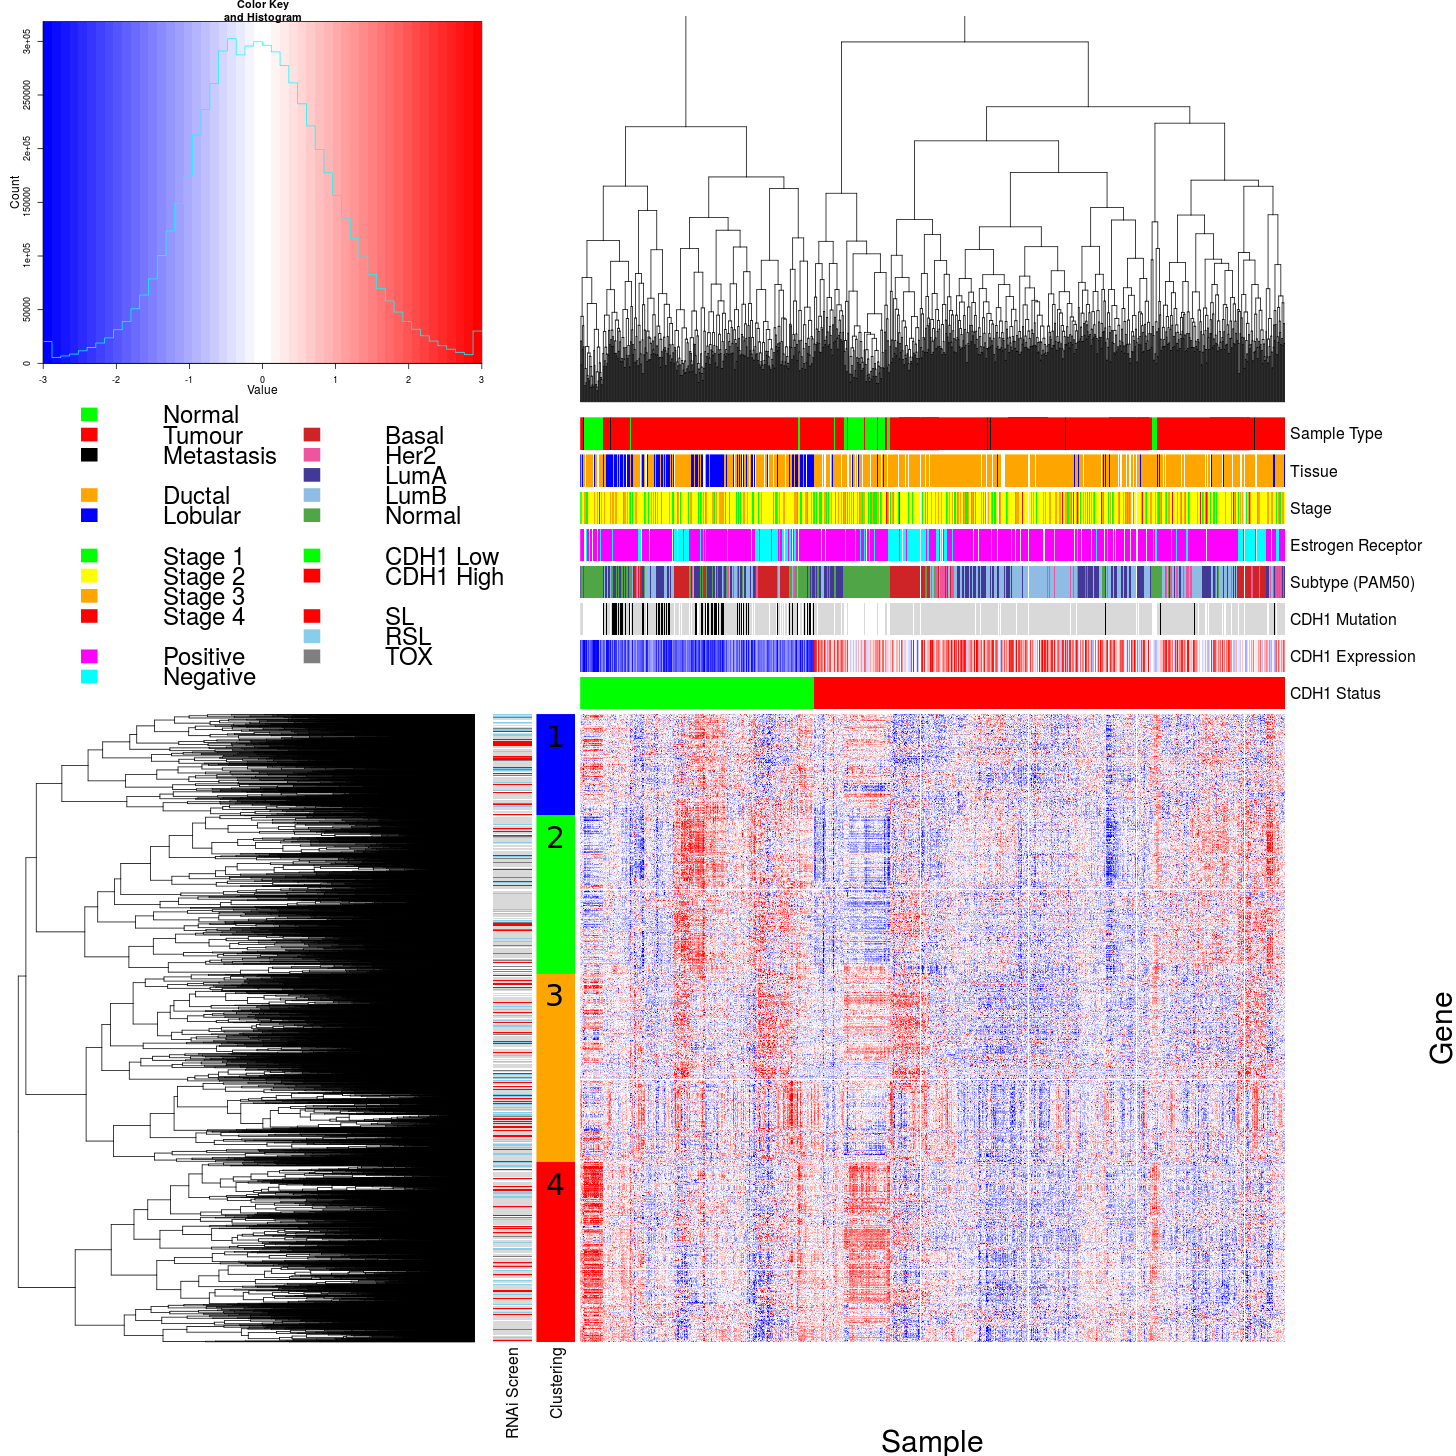
\includegraphics{CDH1_Heatmaps_Genes_Split_By_CDH1_z-trans_exprSL_cordistx_Pub.png}
   }
    \caption[Synthetic lethal expression profiles of analysed samples]{\small \textbf{Synthetic lethal expression profiles of analysed samples.} Gene expression profile heatmap (correlation distance) of all samples (separated by the $\sfrac{1}{3}$ quantile of \textit{CDH1} expression) analysed in TCGA breast cancer dataset for gene expression of 4,629 candidate partners of E-cadherin (\textit{CDH1}) from SLIPT prediction (with significant FDR adjusted $p < 0.05$). Deeply clustered, inter-correlated genes form several main groups, each containing genes that were SL candidates or toxic in an siRNA screen \cite{Telford2015}. Clusters had different sample groups highly expressing the synthetic lethal candidates in \textit{CDH1} low samples, notably 'normal-like', basal, and estrogen receptor negative samples have elevated expression in one or more distinct clusters showing complexity and variation among candidate synthetic lethal partners. \textit{CDH1} low samples also contained most of samples with \textit{CDH1} mutations.
   %This suggests that multiple targets may be needed to target \textit{CDH1} deficiency across genetic backgrounds and that combination therapy may be more effective. 
}
\label{fig:slipt_expr}
\end{mdframed}
\end{figure*}



\begin{table*}[!Hp]
\caption{Pathway composition for clusters of \textit{CDH1} partners from SLIPT}
\label{tab:pathway_clusters}
\centering
\resizebox{0.825 \textwidth}{!}{
\begin{tabular}{sl^c^c^c}
\rowstyle{\bfseries \large}
  \cellcolor{white} Pathways Over-represented in Cluster 1 & Total Genes in Pathway & Genes in SL Cluster & p-val (FDR) \\ %(833 genes)  
  \hline
  \rowcolor{Cluster_Blue!20}
  Collagen formation &  67 &  10 & $4.0 \times 10^{-11}$ \\
  \rowcolor{Cluster_Blue!15} 
  Extracellular matrix organisation & 238 &  21 & $1.8 \times 10^{-9}$ \\
  \rowcolor{Cluster_Blue!20} 
  Collagen biosynthesis and modifying enzymes &  56 &   8 & $1.8 \times 10^{-9}$ \\
  \rowcolor{Cluster_Blue!15} 
  Uptake and actions of bacterial toxins &  22 &   5 & $9.5 \times 10^{-9}$ \\
  \rowcolor{Cluster_Blue!20} 
  Elastic fibre formation &  37 &   6 & $1.9 \times 10^{-8}$ \\
  \rowcolor{Cluster_Blue!15} 
  Muscle contraction &  62 &   7 & $2.4 \times 10^{-7}$ \\
  \rowcolor{Cluster_Blue!20} 
  Fatty acid, triacylglycerol, and ketone body metabolism & 117 &  10 & $4.9 \times 10^{-7}$ \\
  \rowcolor{Cluster_Blue!15} 
  XBP1(S) activates chaperone genes &  51 &   6 & $6.6 \times 10^{-7}$ \\
  \rowcolor{Cluster_Blue!20} 
  IRE1alpha activates chaperones &  54 &   6 & $1.2 \times 10^{-6}$ \\
  \rowcolor{Cluster_Blue!15} 
  Neurotoxicity of clostridium toxins &  10 &   3 & $1.3 \times 10^{-6}$ \\
  \rowcolor{Cluster_Blue!20} 
  Retrograde neurotrophin signalling &  10 &   3 & $1.3 \times 10^{-6}$ \\
  \rowcolor{Cluster_Blue!15} 
  Assembly of collagen fibrils and other multimeric structures &  40 &   5 & $1.9 \times 10^{-6}$ \\
  \rowcolor{Cluster_Blue!20} 
  Collagen degradation &  58 &   6 & $2.0 \times 10^{-6}$ \\
  \rowcolor{Cluster_Blue!15} 
  Arachidonic acid metabolism &  41 &   5 & $2.1 \times 10^{-6}$ \\
  \rowcolor{Cluster_Blue!20} 
  Synthesis of PA &  26 &   4 & $3.0 \times 10^{-6}$ \\
  \rowcolor{Cluster_Blue!15} 
  Signaling by NOTCH &  80 &   7 & $3.3 \times 10^{-6}$ \\
  \rowcolor{Cluster_Blue!20} 
  Signalling to RAS &  27 &   4 & $3.7 \times 10^{-6}$ \\
  \rowcolor{Cluster_Blue!15} 
  Integrin cell surface interactions &  82 &   7 & $4.2 \times 10^{-6}$ \\
  \rowcolor{Cluster_Blue!20} 
  Smooth Muscle Contraction &  28 &   4 & $4.4 \times 10^{-6}$ \\
  %\rowcolor{Cluster_Blue!15} 
  %ECM proteoglycans &  66 &   6 & $6.3 \times 10^{-6}$ \\ 
  \hline
  \\
  \rowstyle{\bfseries \large}
  \cellcolor{white}
  Pathways Over-represented in Cluster 2 & Total Genes in Pathway & Genes in SL Cluster & p-val (FDR) \\ %(1307 genes) 
  \hline
  \rowcolor{Cluster_Green!20}
  Eukaryotic Translation Elongation &  86 &  75 & $1.1 \times 10^{-181}$ \\
  \rowcolor{Cluster_Green!15} 
  Viral mRNA Translation &  81 &  72 & $9.8 \times 10^{-179}$ \\
  \rowcolor{Cluster_Green!20} 
  Peptide chain elongation &  83 &  72 & $1.9 \times 10^{-175}$ \\
  \rowcolor{Cluster_Green!15} 
  Eukaryotic Translation Termination &  83 &  72 & $1.9 \times 10^{-175}$ \\
  \rowcolor{Cluster_Green!20} 
  Formation of a pool of free 40S subunits &  93 &  75 & $1.9 \times 10^{-171}$ \\
  \rowcolor{Cluster_Green!15} 
  Nonsense Mediated Decay (NMD) independent of the Exon Junction Complex (EJC) &  88 &  72 & $9.9 \times 10^{-168}$ \\
  \rowcolor{Cluster_Green!20} 
  L13a-mediated translational silencing of Ceruloplasmin expression & 103 &  75 & $3.0 \times 10^{-159}$ \\
  \rowcolor{Cluster_Green!15} 
  3' -UTR-mediated translational regulation & 103 &  75 & $3.0 \times 10^{-159}$ \\
  \rowcolor{Cluster_Green!20} 
  Nonsense-Mediated Decay (NMD) & 103 &  75 & $3.0 \times 10^{-159}$ \\
  \rowcolor{Cluster_Green!15} 
  Nonsense Mediated Decay (NMD) enhanced by the Exon Junction Complex (EJC) & 103 &  75 & $3.0 \times 10^{-159}$ \\
  \rowcolor{Cluster_Green!20} 
  SRP-dependent cotranslational protein targeting to membrane & 104 &  75 & $3.2 \times 10^{-158}$ \\
  \rowcolor{Cluster_Green!15} 
  GTP hydrolysis and joining of the 60S ribosomal subunit & 104 &  75 & $3.2 \times 10^{-158}$ \\
  \rowcolor{Cluster_Green!20} 
  Eukaryotic Translation Initiation & 111 &  75 & $4.5 \times 10^{-151}$ \\
  \rowcolor{Cluster_Green!15} 
  Cap-dependent Translation Initiation & 111 &  75 & $4.5 \times 10^{-151}$ \\
  \rowcolor{Cluster_Green!20} 
  Influenza Infection & 117 &  75 & $1.4 \times 10^{-145}$ \\
  \rowcolor{Cluster_Green!15} 
  Influenza Viral RNA Transcription and Replication & 108 &  72 & $5.7 \times 10^{-145}$ \\
  \rowcolor{Cluster_Green!20} 
  Translation & 141 &  81 & $8.0 \times 10^{-143}$ \\
  \rowcolor{Cluster_Green!15} 
  Influenza Life Cycle & 112 &  72 & $2.3 \times 10^{-141}$ \\
  \rowcolor{Cluster_Green!20} 
  Infectious disease & 347 & 103 & $2.2 \times 10^{-95}$ \\
  %\rowcolor{Cluster_Green!15} 
  %Formation of the ternary complex, and subsequently, the 43S complex &  47 &  33 & $6.8 \times 10^{-80}$ \\
  \hline
  \\
  \rowstyle{\bfseries \large}
  \cellcolor{white}
  Pathways Over-represented in Cluster 3 & Total Genes in Pathway & Genes in SL Cluster & p-val (FDR) \\ %(1547 genes) 
  \hline
  \rowcolor{Cluster_Orange!30}
  Adaptive Immune System & 412 &  90 & $6.1 \times 10^{-61}$ \\
  \rowcolor{Cluster_Orange!20} 
  Chemokine receptors bind chemokines &  52 &  27 & $6.7 \times 10^{-56}$ \\
  \rowcolor{Cluster_Orange!30} 
  Generation of second messenger molecules &  29 &  21 & $6.5 \times 10^{-55}$ \\
  \rowcolor{Cluster_Orange!20} 
  Immunoregulatory interactions between a Lymphoid and a non-Lymphoid cell &  64 &  29 & $6.5 \times 10^{-55}$ \\
  \rowcolor{Cluster_Orange!30} 
  TCR signalling &  62 &  27 & $8.9 \times 10^{-51}$ \\
  \rowcolor{Cluster_Orange!20} 
  Peptide ligand-binding receptors & 161 &  40 & $1.5 \times 10^{-45}$ \\
  \rowcolor{Cluster_Orange!30} 
  Translocation of ZAP-70 to Immunological synapse &  16 &  14 & $3.1 \times 10^{-43}$ \\
  \rowcolor{Cluster_Orange!20} 
  Costimulation by the CD28 family &  51 &  22 & $4.0 \times 10^{-43}$ \\
  \rowcolor{Cluster_Orange!30} 
  PD-1 signalling &  21 &  15 & $4.0 \times 10^{-41}$ \\
  \rowcolor{Cluster_Orange!20} 
  Class A/1 (Rhodopsin-like receptors) & 258 &  50 & $6.7 \times 10^{-41}$ \\
  \rowcolor{Cluster_Orange!30} 
  Phosphorylation of CD3 and TCR zeta chains &  18 &  14 & $1.3 \times 10^{-40}$ \\
  \rowcolor{Cluster_Orange!20} 
  Interferon gamma signalling &  74 &  24 & $5.0 \times 10^{-39}$ \\
  \rowcolor{Cluster_Orange!30} 
  GPCR ligand binding & 326 &  57 & $1.8 \times 10^{-38}$ \\
  \rowcolor{Cluster_Orange!20} 
  Cytokine Signaling in Immune system & 268 &  48 & $8.9 \times 10^{-37}$ \\
  \rowcolor{Cluster_Orange!30} 
  Downstream TCR signalling &  45 &  18 & $1.8 \times 10^{-35}$ \\
  \rowcolor{Cluster_Orange!20} 
  G$_{\alpha i}$ signalling events & 167 &  33 & $2.2 \times 10^{-33}$ \\
  \rowcolor{Cluster_Orange!30} 
  Cell surface interactions at the vascular wall &  99 &  21 & $1.3 \times 10^{-26}$ \\
  \rowcolor{Cluster_Orange!20} 
  Interferon Signalling & 164 &  28 & $1.7 \times 10^{-26}$ \\
  \rowcolor{Cluster_Orange!30} 
  Extracellular matrix organisation & 238 &  35 & $2.7 \times 10^{-25}$ \\
  %\rowcolor{Cluster_Orange!20} 
  %Antigen activates B Cell Receptor (BCR) leading to generation of second messengers &  32 &  12 & $7.2 \times 10^{-25}$ \\
   \hline
   \\
  \rowstyle{\bfseries \large}
  \cellcolor{white}
  Pathways Over-represented in Cluster 4 & Total Genes in Pathway & Genes in SL Cluster & p-val (FDR) \\ % (1478 genes) 
  \hline
  \rowcolor{Cluster_Red!20}
  Extracellular matrix organisation & 238 &  48 & $8.0 \times 10^{-41}$ \\
  \rowcolor{Cluster_Red!15} 
  Class A/1 (Rhodopsin-like receptors) & 258 &  47 & $2.8 \times 10^{-36}$ \\
  \rowcolor{Cluster_Red!20} 
  GPCR ligand binding & 326 &  54 & $2.1 \times 10^{-34}$ \\
  \rowcolor{Cluster_Red!15} 
  G$_{\alpha s}$ signalling events &  83 &  22 & $1.4 \times 10^{-31}$ \\
  \rowcolor{Cluster_Red!20} 
  GPCR downstream signalling & 472 &  68 & $1.1 \times 10^{-29}$ \\
  \rowcolor{Cluster_Red!15} 
  Haemostasis & 423 &  61 & $3.3 \times 10^{-29}$ \\
  \rowcolor{Cluster_Red!20} 
  Platelet activation, signalling and aggregation & 180 &  31 & $7.1 \times 10^{-28}$ \\
  \rowcolor{Cluster_Red!15} 
  Binding and Uptake of Ligands by Scavenger Receptors &  40 &  14 & $9.9 \times 10^{-27}$ \\
  \rowcolor{Cluster_Red!20} 
  RA biosynthesis pathway &  22 &  11 & $2.5 \times 10^{-26}$ \\
  \rowcolor{Cluster_Red!15} 
  Response to elevated platelet cytosolic Ca$^{2+}$ &  82 &  19 & $3.0 \times 10^{-26}$ \\
  \rowcolor{Cluster_Red!20} 
  Developmental Biology & 420 &  57 & $3.5 \times 10^{-26}$ \\
  \rowcolor{Cluster_Red!15} 
  G$_{\alpha i}$ signalling events & 167 &  28 & $7.3 \times 10^{-26}$ \\
  \rowcolor{Cluster_Red!20} 
  Platelet degranulation &  77 &  18 & $1.6 \times 10^{-25}$ \\
  \rowcolor{Cluster_Red!15} 
  Gastrin-CREB signalling pathway via PKC and MAPK & 171 &  28 & $2.5 \times 10^{-25}$ \\
  \rowcolor{Cluster_Red!20} 
  Muscle contraction &  62 &  16 & $4.7 \times 10^{-25}$ \\
  \rowcolor{Cluster_Red!15} 
  G$_{\alpha q}$ signalling events & 150 &  25 & $3.2 \times 10^{-24}$ \\
  \rowcolor{Cluster_Red!20} 
  Retinoid metabolism and transport &  34 &  12 & $5.0 \times 10^{-24}$ \\
  \rowcolor{Cluster_Red!15} 
  Phase 1 - Functionalisation of compounds &  67 &  16 & $6.5 \times 10^{-24}$ \\
  \rowcolor{Cluster_Red!20} 
  Signalling by Retinoic Acid &  42 &  13 & $6.7 \times 10^{-24}$ \\
  %\rowcolor{Cluster_Red!15} 
  %Degradation of the extracellular matrix & 102 &  19 & $1.4 \times 10^{-22}$ \\ 
  \hline
\end{tabular}
}
\end{table*}



Table 5.  Gene set enrichment results for subgroups of \textit{CDH1} SL partners shows functional variation.

Figure 3.   Heatmap of RNASeq gene expression in predicted SL partners of \textit{CDH1} showing distinct subgroups of SL partners and links between SL partner expression and clinical variables.

\subsubsection{Subgroup pathway analysis}

As discussed previously, \textit{CDH1} (also known as E-Cadherin) is a tumour suppressor gene and the subject of ongoing investigations in the Cancer Genetics Laboratory. Synthetic lethal gene candidates for \textit{CDH1} from RNA-Seq expression data have been the subject of most of my PhD beginning with replication of previous pathway over-representation analyses in RNA-Seq data \citep{genesetdb}.  A novel finding compared to previous analyses in microarray data was correlation structure in the expression of candidates synthetic lethal genes in \textit{CDH1} low tumours (lowest $\sfrac{1}{3}$\textsuperscript{rd} quantile of expression). Subgroups of genes were enriched for distinct biological pathways and elevated in different clusters of samples including some by clinical factors such as estrogen receptor status.

More recent analyses have also investigated intrinsic (PAM50) subtype and somatic mutation (of highest impact genes) against these gene clusters.

\section{Comparison of synthetic lethal gene candidates}

\subsection{Comparison with differential expression}

\subsection{Comparison with correlation}

\subsection{Comparison with primary siRNA screen candidates}


\begin{figure}[!ht]
\begin{mdframed}
  \centering
  \resizebox{0.66 \columnwidth}{!}{
    \includegraphics{Venn_exprSL_siRNA_allgenes_reduced_Pub.png}
   }
    \caption[Comparison of SLIPT to siRNA]{\small \textbf{Comparison of SLIPT to siRNA.} Testing the overlap of gene candidates for E-cadherin synthetic lethal partners between computational (SLIPT) and experimental screening (siRNA) approaches. The $\chi^2$ test suggests that the overlap is no more than would be expected by chance ($p = 0.281$). %A Venn diagram of all 16298 genes tested by both approaches.
}
\label{fig:Venn_allgenes}
\end{mdframed}
\end{figure}

\begin{figure}[!ht]
\begin{mdframed}
  \centering
  \resizebox{0.66 \columnwidth}{!}{
    \includegraphics{Venn_mtSL_siRNA_allgenes_reduced_Pub.png}
   }
    \caption[Comparison of mtSLIPT to siRNA]{\small \textbf{Comparison of mtSLIPT to siRNA.} Testing the overlap of gene candidates for E-cadherin synthetic lethal partners between computational (SLIPT) and experimental screening (siRNA) approaches. The $\chi^2$ test suggests that the overlap is no more than would be expected by chance ($p = 0.281$). %A Venn diagram of all 16298 genes tested by both approaches.
}
\label{fig:Venn_allgenes_mtSL}
\end{mdframed}
\end{figure}

The overlap between synthetic lethal from bioinformatics SLIPT predictions and siRNA screening has raised other questions including whether the number of genes and pathways enriched would be expected by chance. This of particular concern since the siRNA candidate genes themselves are highly enriched for particular pathways so selecting any intersect with them would be enriched for these pathways. The siRNA data is also based on cell line models which have limitations in application to a genetically variable patient population with a complex tumour microenvironment interacting with immune cells. One approach is to compare the candidate genes is to exclude genes that were not tested in both systems, such as those not expressed in cell lines or those with more than $\sfrac{1}{3}$ of TCGA patients without any RNA Seq reads so the lowest quantile cannot be defined for SLIPT analysis. Another approach is to test whether pathways are enriched in randomly sampled genes, comparing many “resampled” or “permutations” of these genes to the enrichment statistics observed for these pathways in the SLIPT candidates and their intersection with the siRNA hits shows whether we detect these pathways more than we expect by chance.

Both of these are being applied with developing a method and overcoming technical challenges for the latter being the focus of recent work. The main challenge at the moment is to compare SLIPT results to experimental candidates and explain why so few genes (and so many pathways) overlap.

As discussed above, comparing genes between experimental screen candidates and prediction from TCGA expression data has been difficult. Figure 3 summarises the approaches to comparing genes accounting for some of the differences between the datasets. Of particular concern are the over-represented pathways in genes detected by both methods. There is no statistical evidence that SLIPT predicted genes or siRNA candidates are enriched in with each other. The siRNA candidates themselves are over-represented with many pathways including GPCRs so any intersection with these would contain some of these pathways. Whether these pathways are contained in the intersection more than expected by chance is the problem the two approaches below were designed to tackle.

\subsubsection{Comparison of screen at pathway level}


\begin{table*}[!Hp]
\caption{Pathway composition for \textit{CDH1} partners from SLIPT and siRNA screening}
\label{tab:Venn_over-representation}
\centering
\resizebox{1 \textwidth}{!}{
\begin{tabular}{sl^c^c^c}
\rowstyle{\bfseries \large}
  Predicted only by SLIPT (4025 genes) & Total Genes in Pathway & Genes Identified & p-val (FDR) \\ 
  \hline
  \rowcolor{Cluster_Red!20}
  Eukaryotic Translation Elongation &  80 &  75 & $1.5 \times 10^{-182}$ \\
  \rowcolor{Cluster_Red!15} 
  Peptide chain elongation &  77 &  72 & $2.9 \times 10^{-176}$ \\
  \rowcolor{Cluster_Red!20} 
  Viral mRNA Translation &  75 &  70 & $4.9 \times 10^{-172}$ \\
  \rowcolor{Cluster_Red!15} 
  Eukaryotic Translation Termination &  76 &  70 & $5.9 \times 10^{-170}$ \\
  \rowcolor{Cluster_Red!20} 
  Formation of a pool of free 40S subunits &  87 &  74 & $9.5 \times 10^{-166}$ \\
  \rowcolor{Cluster_Red!15} 
  Nonsense Mediated Decay (NMD) independent of the Exon Junction Complex (EJC) &  81 &  70 & $1.2 \times 10^{-160}$ \\
  \rowcolor{Cluster_Red!20} 
  L13a-mediated translational silencing of Ceruloplasmin expression &  97 &  75 & $3.8 \times 10^{-155}$ \\
  \rowcolor{Cluster_Red!15} 
  3' -UTR-mediated translational regulation &  97 &  75 & $3.8 \times 10^{-155}$ \\
  \rowcolor{Cluster_Red!20} 
  GTP hydrolysis and joining of the 60S ribosomal subunit &  98 &  75 & $6.0 \times 10^{-154}$ \\
  \rowcolor{Cluster_Red!15} 
  Nonsense-Mediated Decay (NMD) &  96 &  73 & $5.2 \times 10^{-150}$ \\
  \rowcolor{Cluster_Red!20} 
  Nonsense Mediated Decay (NMD) enhanced by the Exon Junction Complex (EJC) &  96 &  73 & $5.2 \times 10^{-150}$ \\
  \rowcolor{Cluster_Red!15} 
  SRP-dependent cotranslational protein targeting to membrane &  97 &  73 & $7.8 \times 10^{-149}$ \\
  \rowcolor{Cluster_Red!20} 
  Eukaryotic Translation Initiation & 105 &  75 & $4.7 \times 10^{-146}$ \\
  \rowcolor{Cluster_Red!15} 
  Cap-dependent Translation Initiation & 105 &  75 & $4.7 \times 10^{-146}$ \\
  \rowcolor{Cluster_Red!20} 
  Translation & 133 &  83 & $4.0 \times 10^{-142}$ \\
  \rowcolor{Cluster_Red!15} 
  Influenza Viral RNA Transcription and Replication & 102 &  71 & $2.9 \times 10^{-137}$ \\
  \rowcolor{Cluster_Red!20} 
  Influenza Infection & 111 &  74 & $3.7 \times 10^{-137}$ \\
  \rowcolor{Cluster_Red!15} 
  Influenza Life Cycle & 106 &  71 & $2.3 \times 10^{-133}$ \\
  \rowcolor{Cluster_Red!20} 
  Infectious disease & 326 & 125 & $4.2 \times 10^{-120}$ \\
  \rowcolor{Cluster_Red!15} 
  Extracellular matrix organisation & 189 &  77 & $5.4 \times 10^{-95}$ \\
  \hline
  \\
  \rowstyle{\bfseries \large}
  Detected only by siRNA screen (1599 genes) & Total Genes in Pathway & Genes Identified & p-val (FDR) \\ 
  \hline
  \rowcolor{Cluster_Blue!20}
  Class A/1 (Rhodopsin-like receptors) & 282 &  44 & $1.3 \times 10^{-27}$ \\
  \rowcolor{Cluster_Blue!15} 
  GPCR ligand binding & 363 &  52 & $5.8 \times 10^{-26}$ \\
  \rowcolor{Cluster_Blue!20} 
  G$_{\alpha q}$ signalling events & 159 &  26 & $6.7 \times 10^{-23}$ \\
  \rowcolor{Cluster_Blue!15} 
  Gastrin-CREB signalling pathway via PKC and MAPK & 180 &  27 & $2.0 \times 10^{-21}$ \\
  \rowcolor{Cluster_Blue!20} 
  G$_{\alpha i}$ signalling events & 184 &  27 & $5.3 \times 10^{-21}$ \\
  \rowcolor{Cluster_Blue!15} 
  Downstream signal transduction & 146 &  23 & $7.6 \times 10^{-21}$ \\
  \rowcolor{Cluster_Blue!20} 
  Signalling by PDGF & 172 &  25 & $4.0 \times 10^{-20}$ \\
  \rowcolor{Cluster_Blue!15} 
  Peptide ligand-binding receptors & 175 &  25 & $8.5 \times 10^{-20}$ \\
  \rowcolor{Cluster_Blue!20} 
  Signalling by ERBB2 & 146 &  22 & $1.3 \times 10^{-19}$ \\
  \rowcolor{Cluster_Blue!15} 
  DAP12 interactions & 159 &  23 & $2.6 \times 10^{-19}$ \\
  \rowcolor{Cluster_Blue!20} 
  DAP12 signalling & 149 &  22 & $2.7 \times 10^{-19}$ \\
  \rowcolor{Cluster_Blue!15} 
  Organelle biogenesis and maintenance & 264 &  33 & $5.5 \times 10^{-19}$ \\
  \rowcolor{Cluster_Blue!20} 
  Signalling by NGF & 266 &  33 & $8.2 \times 10^{-19}$ \\
  \rowcolor{Cluster_Blue!15} 
  Downstream signalling of activated FGFR1 & 134 &  20 & $1.1 \times 10^{-18}$ \\
  \rowcolor{Cluster_Blue!20} 
  Downstream signalling of activated FGFR2 & 134 &  20 & $1.1 \times 10^{-18}$ \\
  \rowcolor{Cluster_Blue!15} 
  Downstream signalling of activated FGFR3 & 134 &  20 & $1.1 \times 10^{-18}$ \\
  \rowcolor{Cluster_Blue!20} 
  Downstream signalling of activated FGFR4 & 134 &  20 & $1.1 \times 10^{-18}$ \\
  \rowcolor{Cluster_Blue!15} 
  Signalling by FGFR & 146 &  21 & $1.3 \times 10^{-18}$ \\
  \rowcolor{Cluster_Blue!20} 
  Signalling by FGFR1 & 146 &  21 & $1.3 \times 10^{-18}$ \\
  \rowcolor{Cluster_Blue!15} 
  Signalling by FGFR2 & 146 &  21 & $1.3 \times 10^{-18}$ \\
  \hline
  \\
  \rowstyle{\bfseries \large}
  Intersection of SLIPT and siRNA screen (604 genes) & Total Genes in Pathway & Genes Identified & p-val (FDR) \\ 
  \hline
  \rowcolor{Cluster_Red!20!Cluster_Blue!20}
  Visual phototransduction &  54 &   9 & $6.9 \times 10^{-10}$ \\
  \rowcolor{Cluster_Red!15!Cluster_Blue!15} 
  G$_{\alpha s}$ signalling events &  48 &   7 & $1.6 \times 10^{-7}$ \\
  \rowcolor{Cluster_Red!20!Cluster_Blue!20} 
  Retinoid metabolism and transport &  24 &   5 & $1.7 \times 10^{-7}$ \\
  \rowcolor{Cluster_Red!15!Cluster_Blue!15} 
  Acyl chain remodelling of PS &  10 &   3 & $6.5 \times 10^{-6}$ \\
  \rowcolor{Cluster_Red!20!Cluster_Blue!20} 
  Transcriptional regulation of white adipocyte differentiation &  51 &   6 & $6.5 \times 10^{-6}$ \\
  \rowcolor{Cluster_Red!15!Cluster_Blue!15} 
  Chemokine receptors bind chemokines &  22 &   4 & $6.5 \times 10^{-6}$ \\
  \rowcolor{Cluster_Red!20!Cluster_Blue!20} 
  Signalling by NOTCH4 &  11 &   3 & $6.9 \times 10^{-6}$ \\
  \rowcolor{Cluster_Red!15!Cluster_Blue!15} 
  Defective EXT2 causes exostoses 2 &  11 &   3 & $6.9 \times 10^{-6}$ \\
  \rowcolor{Cluster_Red!20!Cluster_Blue!20} 
  Defective EXT1 causes exostoses 1, TRPS2 and CHDS &  11 &   3 & $6.9 \times 10^{-6}$ \\
  \rowcolor{Cluster_Red!15!Cluster_Blue!15} 
  Platelet activation, signalling and aggregation & 146 &  12 & $6.9 \times 10^{-6}$ \\
  \rowcolor{Cluster_Red!20!Cluster_Blue!20} 
  Phase 1 - Functionalisation of compounds &  41 &   5 & $1.3 \times 10^{-5}$ \\
  \rowcolor{Cluster_Red!15!Cluster_Blue!15} 
  Amine ligand-binding receptors &  13 &   3 & $1.7 \times 10^{-5}$ \\
  \rowcolor{Cluster_Red!20!Cluster_Blue!20} 
  Acyl chain remodelling of PE &  14 &   3 & $2.4 \times 10^{-5}$ \\
  \rowcolor{Cluster_Red!15!Cluster_Blue!15} 
  Signalling by GPCR & 300 &  23 & $2.4 \times 10^{-5}$ \\
  \rowcolor{Cluster_Red!20!Cluster_Blue!20} 
  Molecules associated with elastic fibres &  29 &   4 & $2.6 \times 10^{-5}$ \\
  \rowcolor{Cluster_Red!15!Cluster_Blue!15} 
  DAP12 interactions & 128 &  10 & $2.6 \times 10^{-5}$ \\
  \rowcolor{Cluster_Red!20!Cluster_Blue!20} 
  Cytochrome P$_{450}$ - arranged by substrate type &  30 &   4 & $3.2 \times 10^{-5}$ \\
  \rowcolor{Cluster_Red!15!Cluster_Blue!15} 
  GPCR ligand binding & 147 &  11 & $3.8 \times 10^{-5}$ \\
  \rowcolor{Cluster_Red!20!Cluster_Blue!20} 
  Acyl chain remodelling of PC &  16 &   3 & $4.0 \times 10^{-5}$ \\
  \rowcolor{Cluster_Red!15!Cluster_Blue!15} 
  Response to elevated platelet cytosolic Ca$^{2+}$ &  66 &   6 & $4.2 \times 10^{-5}$ \\ 
  \hline
\end{tabular}
}
\end{table*}



\subsubsubsection{Resampling of genes for pathway enrichment}

\begin{figure}[!ht]
\begin{mdframed}
  \centering
  \resizebox{0.66 \columnwidth}{!}{
    \includegraphics{sample_size_dist_exprSL_1M_Pub.png}
   }
   \caption[Expected distribution of sample size for intersect with siRNA candidates]{\small \textbf{Expected distribution of sample size for intersect with siRNA candidates.} Resampling analysis of intersect size from genes detected by SLIPT and siRNA screening approaches over 1 million replicates. The proportion of expected intersection sizes for random samples below or above the observed intersection size respectively, lacking significant over-represent\-ation or depletion of siRNA screen candidates within the SLIPT predictions for \textit{CDH1}.
   %However, the pathway composition of this intersect may still be informative. %%covered in text
}
\label{fig:perm_sample}
\end{mdframed}
\end{figure}


\begin{table*}[!Htp]
\caption{Pathway Analysis of \textit{CDH1} partners from SLIPT}
\label{tab:pathway_perm}
\centering
\resizebox{1 \textwidth}{!}{
\begin{tabular}{sl^c^c^c}
\rowstyle{\bfseries \large}
 Reactome Pathway & Over-representation (FDR p-val) & Permutation (FDR p-val) \\ 
  \hline
  \rowcolor{Cluster_Red!20} 
  \textbf{Eukaryotic Translation Elongation} & $1.3 \times 10^{-207}$ & $< 1.241 \times 10^{-5}$  \\
  \rowcolor{Cluster_Red!15}  
   \textbf{Peptide chain elongation} & $5.6 \times 10^{-201}$ & $< 1.241 \times 10^{-5}$  \\
  \rowcolor{Cluster_Red!20}  
   \textbf{Viral mRNA Translation} & $1.2 \times 10^{-196}$ & $< 1.241 \times 10^{-5}$  \\
  \rowcolor{Cluster_Red!15}  
   \textbf{Eukaryotic Translation Termination} & $1.2 \times 10^{-196}$ & $< 1.241 \times 10^{-5}$  \\
  \rowcolor{Cluster_Red!20}  
   \textbf{Formation of a pool of free 40S subunits} & $3.7 \times 10^{-194}$ & $< 1.241 \times 10^{-5}$  \\
  \rowcolor{Cluster_Red!15}  
   \textbf{Nonsense Mediated Decay (NMD) independent of the Exon Junction Complex (EJC)} & $5.3 \times 10^{-187}$ & $< 1.241 \times 10^{-5}$  \\
  \rowcolor{Cluster_Red!20}  
   \textbf{L13a-mediated translational silencing of Ceruloplasmin expression} & $9.6 \times 10^{-183}$ & $< 1.241 \times 10^{-5}$  \\
  \rowcolor{Cluster_Red!15}  
   \textbf{3' -UTR-mediated translational regulation} & $9.6 \times 10^{-183}$ & $< 1.241 \times 10^{-5}$  \\
  \rowcolor{Cluster_Red!20}  
   \textbf{GTP hydrolysis and joining of the 60S ribosomal subunit} & $1.9 \times 10^{-181}$ & $< 1.241 \times 10^{-5}$  \\
  \rowcolor{Cluster_Red!15}  
   \textbf{Nonsense-Mediated Decay (NMD)} & $6.2 \times 10^{-176}$ & $< 1.241 \times 10^{-5}$  \\
  \rowcolor{Cluster_Red!20}  
   \textbf{Nonsense Mediated Decay (NMD) enhanced by the Exon Junction Complex (EJC)} & $6.2 \times 10^{-176}$ & $< 1.241 \times 10^{-5}$  \\
  \rowcolor{Cluster_Red!15}  
  Adaptive Immune System & $6.5 \times 10^{-174}$ & $0.15753$ \\
  \rowcolor{Cluster_Red!20}  
  \textbf{Eukaryotic Translation Initiation} & $5.7 \times 10^{-173}$ & $< 1.241 \times 10^{-5}$  \\
  \rowcolor{Cluster_Red!15}  
  \textbf{Cap-dependent Translation Initiation} & $5.7 \times 10^{-173}$ & $< 1.241 \times 10^{-5}$  \\
  \rowcolor{Cluster_Red!20}  
  \textbf{SRP-dependent cotranslational protein targeting to membrane} & $2.0 \times 10^{-171}$ & $< 1.241 \times 10^{-5}$  \\
  \rowcolor{Cluster_Red!15}  
  \textbf{Translation} & $6.1 \times 10^{-170}$ & $< 1.241 \times 10^{-5}$  \\
  \rowcolor{Cluster_Red!20}  
  Infectious disease & $1.6 \times 10^{-166}$ & $0.23231$ \\
  \rowcolor{Cluster_Red!15}  
  \textbf{Influenza Infection} & $1.9 \times 10^{-163}$ & $< 1.241 \times 10^{-5}$  \\
  \rowcolor{Cluster_Red!20}  
  \textbf{Influenza Viral RNA Transcription and Replication} & $1.9 \times 10^{-160}$ & $< 1.241 \times 10^{-5}$  \\
  \rowcolor{Cluster_Red!15}  
  \textbf{Influenza Life Cycle} & $2.5 \times 10^{-156}$ & $< 1.241 \times 10^{-5}$  \\
  \rowcolor{Cluster_Red!20}  
  Extracellular matrix organisation & $1.1 \times 10^{-152}$ & $0.071761$ \\
  \rowcolor{Cluster_Red!15}  
  GPCR ligand binding & $1.1 \times 10^{-143}$ & $0.55801$ \\
  \rowcolor{Cluster_Red!20}  
  Class A/1 (Rhodopsin-like receptors) & $1.5 \times 10^{-142}$ & $0.58901$ \\
  \rowcolor{Cluster_Red!15}  
  GPCR downstream signalling & $7.6 \times 10^{-140}$ & $0.098357$ \\
  \rowcolor{Cluster_Red!20}  
  Haemostasis & $1.9 \times 10^{-134}$ & $0.27059$ \\
  \rowcolor{Cluster_Red!15}  
  Developmental Biology & $2.0 \times 10^{-123}$ & $0.52737$ \\
  \rowcolor{Cluster_Red!20}  
  Metabolism of lipids and lipoproteins & $3.3 \times 10^{-120}$ & $0.724$ \\
  \rowcolor{Cluster_Red!15}  
  Cytokine Signalling in Immune system & $2.6 \times 10^{-119}$ & $0.39661$ \\
  \rowcolor{Cluster_Red!20}  
  Peptide ligand-binding receptors & $3.7 \times 10^{-109}$ & $0.61102$ \\
  \rowcolor{Cluster_Red!15}  
  \textbf{G$_{\alpha i}$ signalling events} & $8.9 \times 10^{-100}$ & $< 1.241 \times 10^{-5}$  \\
  \iffalse
  \rowcolor{Cluster_Red!20}  
  Axon guidance & $1.4 \times 10^{-96}$ & $0.66232$ \\
  \rowcolor{Cluster_Red!15}  
  Platelet activation, signalling and aggregation & $3.7 \times 10^{-94}$ & $0.29662$ \\
  \rowcolor{Cluster_Red!20}  
  Immunoregulatory interactions between a Lymphoid and a non-Lymphoid cell & $1.4 \times 10^{-93}$ & $< 1.241 \times 10^{-5}$  \\
  \rowcolor{Cluster_Red!15}  
  Formation of the ternary complex, and subsequently, the 43S complex & $7.0 \times 10^{-91}$ & $< 1.241 \times 10^{-5}$  \\
  \rowcolor{Cluster_Red!20}  
  Translation initiation complex formation & $9.6 \times 10^{-87}$ & $6.8667 \times 10^{-5}$  \\
  \rowcolor{Cluster_Red!15}  
  Ribosomal scanning and start codon recognition & $9.6 \times 10^{-87}$ & $6.8667 \times 10^{-5}$  \\
  \rowcolor{Cluster_Red!20}  
  Activation of the mRNA upon binding of the cap-binding complex and eIFs, and subsequent binding to 43S & $8.7 \times 10^{-86}$ & $6.8667 \times 10^{-5}$  \\
  \rowcolor{Cluster_Red!15}  
  Chemokine receptors bind chemokines & $5.1 \times 10^{-82}$ & $< 1.241 \times 10^{-5}$  \\
  \rowcolor{Cluster_Red!20}  
  Signalling by NGF & $1.2 \times 10^{-81}$ & $0.37142$ \\
  \rowcolor{Cluster_Red!15}  
  Toll-Like Receptors Cascades & $5.3 \times 10^{-80}$ & $0.63013$ \\
  \rowcolor{Cluster_Red!20}  
  Interferon gamma signalling & $6.3 \times 10^{-80}$ & $0.61493$ \\
  \rowcolor{Cluster_Red!15}  
  Transmembrane transport of small molecules & $5.3 \times 10^{-78}$ & $0.21216$ \\
  \rowcolor{Cluster_Red!20}  
  Signalling by Rho GTPases & $1.1 \times 10^{-77}$ & $0.078314$ \\
  \rowcolor{Cluster_Red!15}  
  Degradation of the extracellular matrix & $7.3 \times 10^{-77}$ & $0.769$ \\
  \rowcolor{Cluster_Red!20}  
  Interferon Signalling & $1.1 \times 10^{-76}$ & $0.18211$ \\
  \rowcolor{Cluster_Red!15}  
  NGF signalling via TRKA from the plasma membrane & $1.4 \times 10^{-74}$ & $0.60076$ \\
  \rowcolor{Cluster_Red!20}  
  Gastrin-CREB signalling pathway via PKC and MAPK & $3.1 \times 10^{-74}$ & $0.93109$ \\
  \rowcolor{Cluster_Red!15}  
  Rho GTPase cycle & $3.2 \times 10^{-73}$ & $0.11446$ \\
  \rowcolor{Cluster_Red!20}  
  DAP12 interactions & $2.0 \times 10^{-71}$ & $0.57671$ \\
  \rowcolor{Cluster_Red!15}  
  Cell surface interactions at the vascular wall & $3.3 \times 10^{-71}$ & $0.66232$ \\ 
  \fi
  \hline
\end{tabular}
}
\end{table*}

\begin{table*}[!Htp]
\caption{Pathway Analysis of \textit{CDH1} partners from SLIPT and siRNA primary screen}
\label{tab:pathway_perm_overlap}
\centering
\resizebox{1 \textwidth}{!}{
\begin{tabular}{sl^c^c^c}
\rowstyle{\bfseries \large}
 Reactome Pathway & Over-representation (FDR) & Permutation (FDR) \\ 
  \hline
  \rowcolor{Cluster_Red!20!Cluster_Blue!20} 
  Visual phototransduction & $6.9 \times 10^{-10}$ & $0.91116$  \\
  \rowcolor{Cluster_Red!15!Cluster_Blue!15}  
  \textbf{G$_{\alpha s}$ signalling events} & $1.6 \times 10^{-7}$ & $0.012988$  \\
  \rowcolor{Cluster_Red!20!Cluster_Blue!20}  
  Retinoid metabolism and transport & $1.7 \times 10^{-7}$ & $0.20487$  \\
  \rowcolor{Cluster_Red!15!Cluster_Blue!15}  
  Transcriptional regulation of white adipocyte differentiation & $6.5 \times 10^{-6}$ & $0.38197$  \\
  \rowcolor{Cluster_Red!20!Cluster_Blue!20}  
  Acyl chain remodelling of PS & $6.5 \times 10^{-6}$ & $0.58485$  \\
  \rowcolor{Cluster_Red!15!Cluster_Blue!15}  
  Chemokine receptors bind chemokines & $6.5 \times 10^{-6}$ & $0.97255$  \\
  \rowcolor{Cluster_Red!20!Cluster_Blue!20}  
  \textit{Defective EXT2 causes exostoses 2} & $6.9 \times 10^{-6}$ & $0.056437$  \\
  \rowcolor{Cluster_Red!15!Cluster_Blue!15}  
  \textit{Defective EXT1 causes exostoses 1, TRPS2 and CHDS} & $6.9 \times 10^{-6}$ & $0.056437$  \\
  \rowcolor{Cluster_Red!20!Cluster_Blue!20}  
  Signalling by NOTCH4 & $6.9 \times 10^{-6}$ & $0.15497$  \\
  \rowcolor{Cluster_Red!15!Cluster_Blue!15}  
  Platelet activation, signalling and aggregation & $6.9 \times 10^{-6}$ & $0.53358$  \\
  \rowcolor{Cluster_Red!20!Cluster_Blue!20}  
  Phase 1 - Functionalisation of compounds & $1.3 \times 10^{-5}$ & $0.24836$  \\
  \rowcolor{Cluster_Red!15!Cluster_Blue!15}  
  Amine ligand-binding receptors & $1.7 \times 10^{-5}$ & $0.3195$  \\
  \rowcolor{Cluster_Red!20!Cluster_Blue!20}  
  Acyl chain remodelling of PE & $2.4 \times 10^{-5}$ & $0.7307$  \\
  \rowcolor{Cluster_Red!15!Cluster_Blue!15}  
  Signalling by GPCR & $2.4 \times 10^{-5}$ & $0.9939$  \\
  \rowcolor{Cluster_Red!20!Cluster_Blue!20}  
  \textbf{Molecules associated with elastic fibres} & $2.6 \times 10^{-5}$ & $0.0072929$  \\
  \rowcolor{Cluster_Red!15!Cluster_Blue!15}  
  DAP12 interactions & $2.6 \times 10^{-5}$ & $0.78273$  \\
  \rowcolor{Cluster_Red!20!Cluster_Blue!20}  
  Cytochrome P$_{450}$ - arranged by substrate type & $3.2 \times 10^{-5}$ & $0.87019$  \\
  \rowcolor{Cluster_Red!15!Cluster_Blue!15}  
  GPCR ligand binding & $3.8 \times 10^{-5}$ & $0.99417$  \\
  \rowcolor{Cluster_Red!20!Cluster_Blue!20}  
  Acyl chain remodelling of PC & $4.0 \times 10^{-5}$ & $0.65415$  \\
  \rowcolor{Cluster_Red!15!Cluster_Blue!15}  
  Response to elevated platelet cytosolic Ca$^{2+}$ & $4.2 \times 10^{-5}$ & $0.55461$  \\
  \rowcolor{Cluster_Red!20!Cluster_Blue!20}  
  \textit{Arachidonic acid metabolism} & $4.4 \times 10^{-5}$ & $0.060298$  \\
  \rowcolor{Cluster_Red!15!Cluster_Blue!15}  
  Defective B4GALT7 causes EDS, progeroid type & $4.9 \times 10^{-5}$ & $0.15497$  \\
  \rowcolor{Cluster_Red!20!Cluster_Blue!20}  
  Defective B3GAT3 causes JDSSDHD & $4.9 \times 10^{-5}$ & $0.15497$  \\
  \rowcolor{Cluster_Red!15!Cluster_Blue!15}  
  \textbf{Elastic fibre formation} & $4.9 \times 10^{-5}$ & $0.0019227$  \\
  \rowcolor{Cluster_Red!20!Cluster_Blue!20}  
  \textbf{HS-GAG degradation} & $6.2 \times 10^{-5}$ & $0.017747$  \\
  \rowcolor{Cluster_Red!15!Cluster_Blue!15}  
  Bile acid and bile salt metabolism & $6.2 \times 10^{-5}$ & $0.15497$  \\
  \rowcolor{Cluster_Red!20!Cluster_Blue!20}  
  Netrin-1 signalling & $7.1 \times 10^{-5}$ & $0.95056$  \\
  \rowcolor{Cluster_Red!15!Cluster_Blue!15}  
  \textbf{Integration of energy metabolism} & $7.1 \times 10^{-5}$ & $0.0019287$  \\
  \rowcolor{Cluster_Red!20!Cluster_Blue!20}  
  DAP12 signalling & $7.9 \times 10^{-5}$ & $0.67835$  \\
  \rowcolor{Cluster_Red!15!Cluster_Blue!15}  
  GPCR downstream signalling & $8.1 \times 10^{-5}$ & $0.88678$  \\
  \rowcolor{Cluster_Red!20!Cluster_Blue!20}  
  \textbf{Diseases associated with glycosaminoglycan metabolism} & $8.7 \times 10^{-5}$ & $0.017747$  \\
  \rowcolor{Cluster_Red!15!Cluster_Blue!15}  
  \textbf{Diseases of glycosylation} & $8.7 \times 10^{-5}$ & $0.017747$  \\
  \rowcolor{Cluster_Red!20!Cluster_Blue!20}  
  Signalling by Retinoic Acid & $8.7 \times 10^{-5}$ & $0.13592$  \\
  \rowcolor{Cluster_Red!15!Cluster_Blue!15}  
  Signalling by Leptin & $8.7 \times 10^{-5}$ & $0.15497$  \\
  \rowcolor{Cluster_Red!20!Cluster_Blue!20}  
  Signalling by SCF-KIT & $8.7 \times 10^{-5}$ & $0.73399$  \\
  \rowcolor{Cluster_Red!15!Cluster_Blue!15}  
  Opioid Signalling & $8.7 \times 10^{-5}$ & $0.99417$  \\
  \rowcolor{Cluster_Red!20!Cluster_Blue!20}  
  Signalling by NOTCH & $0.0001$ & $0.26453$  \\
  \rowcolor{Cluster_Red!15!Cluster_Blue!15}  
  Platelet homeostasis & $0.0001$ & $0.55912$  \\
  \rowcolor{Cluster_Red!20!Cluster_Blue!20}  
  Signalling by NOTCH1 & $0.00011$ & $0.13797$  \\
  \rowcolor{Cluster_Red!15!Cluster_Blue!15}  
  Class B/2 (Secretin family receptors) & $0.00011$ & $0.4659$  \\
  \rowcolor{Cluster_Red!20!Cluster_Blue!20}  
  Diseases of Immune System & $0.00013$ & $0.15497$  \\
  \rowcolor{Cluster_Red!15!Cluster_Blue!15}  
  Diseases associated with the TLR signalling cascade & $0.00013$ & $0.15497$  \\
  \rowcolor{Cluster_Red!20!Cluster_Blue!20}  
  A tetrasaccharide linker sequence is required for GAG synthesis & $0.00013$ & $0.33566$  \\
  \rowcolor{Cluster_Red!15!Cluster_Blue!15}  
  Nuclear Receptor transcription pathway & $0.00016$ & $0.22735$  \\
  \rowcolor{Cluster_Red!20!Cluster_Blue!20}  
  \textbf{Formation of Fibrin Clot (Clotting Cascade)} & $0.00016$ & $0.0054639$  \\
  \rowcolor{Cluster_Red!15!Cluster_Blue!15}  
  Syndecan interactions & $0.00016$ & $0.3974$  \\
  \rowcolor{Cluster_Red!20!Cluster_Blue!20}  
  Class A/1 (Rhodopsin-like receptors) & $0.00016$ & $0.99454$  \\
  \rowcolor{Cluster_Red!15!Cluster_Blue!15}  
  HS-GAG biosynthesis & $0.0002$ & $0.37199$  \\
  \rowcolor{Cluster_Red!20!Cluster_Blue!20}  
  Platelet degranulation  & $0.0002$ & $0.39003$  \\
  \rowcolor{Cluster_Red!15!Cluster_Blue!15}  
  EPH-ephrin mediated repulsion of cells & $0.00021$ & $0.6193$  \\ 
  \hline
\end{tabular}
}
\end{table*}



\subsection{Comparison with secondary screen siRNA screen candidates}

\subsubsection{Comparison of candidate SL Pathways}

Thus we have identified candidate synthetic lethal pathways by gene set over-representation, metagene synthetic lethality, and re-sampled empirical pathway over-representation. The challenge currently under consideration is whether these methods can be compared and which may lead to biologically meaningful or clinically relevant synthetic lethal candidate pathways.

\section{Mutation, Copy Number, and Methylation}

Due to promising synthetic lethal data on mutation and DNA copy number analyses \citep{Jerby2014, Lu2015}, these were also investigated to compare genes for synthetic lethality in an analogous manner to expression analyses in the TCGA data. Due to the low somatic mutation rate (and lack of available) germline mutations for many genes, it was not possible to detect many double mutations with significantly under-representation in cancers. There were also concerns about using rare mutations with unknown significance or excluding functional mutations by only using those in the exons.
It was possible to compare deletion and duplication of DNA copy number in a manner analogous to expression quantiles. However, these overlapped poorly with candidate interacting partners from expression analyses and concerns were raised that they may not be relevant to \textit{CDH1} which is typically inactivated in tumours by loss of function mutations or DNA methylation (PJ Guilford, personal communication).   

DNA methylation data was also prepared for synthetic lethal analysis but was discontinued due to computational challenges, expected similarity to expression results, difficulty defining loss of function methylation at a gene level across CpG sites, and the concerns raised in the next section. 

\subsection{Synthetic lethality by DNA copy number}

\subsection{Synthetic lethality by somatic mutation}

\subsubsection{Mutation analysis}

\subsection{ANOVA of Expression Predictors}
[include?]

Another approach was to only use copy number, mutation, or hyper-methylation data for genes in which they would impact on gene function and occur frequently in tumours. Before investigating whether these impact on gene function, they were investigated as predictors of variation in gene expression. If these are not giving variation independent of gene expression, expression would be a more suitable measure of gene function as it is widely generated in studies and useful as a clinical biomarker.

Globally predicting gene expression across all genes from DNA copy number and somatic mutation was attempted by ANOVA. However, this was computationally challenging and gene-specific analyses would be more informative. Gene specific ANOVA and linear regression was performed but was raised more issues than it addressed. There were issues with interaction terms and mutation data, many genes were not tested for these since there were so few mutations for these genes in the dataset.  It was possible to include DNA methylation in gene-specific analyses (despite the concerns raised above) but the $R^2$ values for each gene were still generally very low and issues with insufficient mutant samples for interaction terms became worse. This means that the approach used differs for each gene making it difficult to compare them. The challenges raised here suggested that expression is very difficult to predict with other factors but including these other factors would be difficult and plagued by multiple-testing, particularly comparing between them with the current synthetic lethal prediction method. This led to investigations into the simulation of synthetic lethality.

\section{Global Synthetic Lethality}
[include?]

Global levels of synthetic lethality were analysed as part of my Honours project to address concerns of high numbers of synthetic lethal candidates for \textit{CDH1}. This turned out to be typical for most genes in the microarray dataset. Due to newer samples and concerns about sample quality in TCGA microarrays, RNA-Seq datasets were used here. The focus of this thesis is gene expression data generated by RNA-Seq, this was replicated using the TCGA breast cancer RNA-Seq dataset on the New Zealand eScience Infrastructure Intel Pan supercomputer.

\subsection{Hub Genes}
Table 1.  Hub gene function in TCGA breast cancer microarray expression SL predictions (n=600).

Table 2 Hub gene function in TCGA breast cancer RNA-Seq expression SL predictions (n=878). [revise for n=1168]

Table 3.  Hub gene function in BC2116 breast cancer microarray expression SL predictions (n=2116).


\section{Metagene Analysis}
[include?]

\subsection{Pathway expression}

\subsection{Somatic mutation}

\subsection{Synthetic lethal metagenes}

\section{Replication in stomach cancer}

\begin{itemize}
 \item exprSL
 \item mtSL
 \item heatmap
 \item Venn
 \item Pathway enrichment
 \item Permutations
\end{itemize}

\section{Replication in cell line encyclopaedia}

As breast cancer cell lines are the experimental system in which many cancer genetics and drug targets are investigated, these were analysed in addition to patient samples from TCGA. The cancer cell line encyclopaedia (CCLE) is a resource for genomics profiles across a range of cell lines. These have also been used to generate synthetic lethal candidates for comparison to those in experimental screen and predictions from TCGA expression data.
A transcriptome experiment has been conducted by the Cancer Genetics Laboratory to test their \textit{CDH1}$^{-/-}$ null MCF10A cell lines compared to an otherwise isogenic wildtype \citep{Chen2014}. While differential expression analysis was inconclusive due to few technical replicates, this data was also useful to determine genes which were not detectable in MCF10A cell lines which would not be expected to detect synthetic lethality in siRNA screen data even if they were predicted to be synthetic lethal in expression data. 


\section{Summary}

We have developed a simple, interpretable, computational approach to predict synthetic lethal partners from genomics data.  Originally developed for microarray gene expression data, it has been expanded to test DNA copy number, or RNA-Seq gene expression data which are both also supported by the TCGA dataset.  DNA copy number was included for comparison with the DAISY tool of \citet{Jerby2014}.  Predictions based on microarray data were inconclusive when compared with an RNAi screen for \textit{CDH1} in MCF10A breast cells as performed by \citet{Telford2015}, few predictions replicated between BC2116, CCLE, or TCGA microarray datasets, results with gene expression and DNA copy number were vastly different, and predictions from TCGA microarray and RNA-Seq datasets for the same samples differed were inconsistent.  The Aligent TCGA microarray data in particular is difficult to compare to other datasets and will in the future use Affymetrix microarrays or RNA-Seq platforms for predictions from gene expression data.  The analyses focus on gene expression data as it is widely available for applications in other cancers and current attempts to use gene expression data for synthetic lethal discovery vary widely \citep{Jerby2014, Lu2015, Tiong2014}.  There is no consensus for which approach is more appropriate since they lack much a basis on biological experimental data or statistical modelling and often use difficult to interpret machine learning methodology.

Genomics analyses are prone to false-positives and require statistical caution, particularly where working with gene-pairs scale up the number of multiple tests drastically, at the expense of statistical power.  Experimental SGA and RNAi screens for synthetic lethality are also error-prone, especially with false-positives, raising the need for understanding the expected behaviour and number of functional relationships and genetic interactions in the genome, or in discovery of synthetic lethal partners of a particular query gene.  A characteristic of gene interaction networks is a scale-free topology leading to highly interacting ‘hub’ genes, these represent important genes in a functional network.  As shown in Tables 1-3, Gene Ontology terms for genes important in cancer proliferation, progression, and drug response were enriched in hub genes, showing that synthetic lethal interactions are among important genes in cancer cells.  Gene functions replicated across the breast cancer datasets are highlighted in bold, despite differences in particular hits, gene expression platforms, and only correcting for multiple tests for each gene query separately, there are many gene functions replicated across breast cancer gene expression analyses.  TCGA microarray data was less consistent with the other datasets, as expected from lower sample size, lower concordance of particular hits for the example query of \textit{CDH1}, and suspected lower quality of data on the Aligent microarray platform.

As specific genes were difficult to replicate across experiments, gene expression profiles for synthetic lethal partners must be more complex than originally expected to directly compensate for loss of query gene or completely lack (or clearly under-represent) co-loss \citep{Kelly2013, Jerby2014, Lu2015}.  The predicted synthetic lethal partners of \textit{CDH1} (with FDR correction) were investigated with gene expression profiles and clinical variables to find relationships in gene expression, gene function, and clinical characteristics.  The large number of hits indicate that synthetic lethality is error-prone and identifying genes or pathways relevant for clinical application will be difficult.

The expression profiles of the SL partners of \textit{CDH1} predicted from the TCGA breast cancer RNA-Seq data in \textit{CDH1} low tumours (where synthetic lethal partners are expected to have compensating high or stable expression) are shown in Figure 7 and their corresponding functional enrichment is given below in Table 5, computed as WikiPathways in GeneSetDB \citep{genesetdb}.  The 3 subgroups of genes are showed functional organisation of expression profiles in \textit{CDH1} low breast tumours.  The first group is enriched for G protein coupled receptors, an established drug target and supported in cell line experiments \citep{Telford2015}.  The second group contains genes involved in development and metabolism consistent with cancer cells showing stem cell properties and the Warburg hypothesis \citep{Merlos-Suarez2011, Warburg1956}.  The third group contains cell signalling and focal adhesion functions, including pathways involved in cancer proliferation, metastasis, and consistent with internal synthetic lethality within the pathways containing \textit{CDH1} \citep{Barabasi2004}.

Ductal breast cancers show higher expression of synthetic lethal partners suggesting treatment would be more effective in this tumour subtype.  However, there is consistently low expression of SL partners in ER negative tumours, although this is independent of tumour stage and consistent with poor prognosis in these patients and could inform other treatment strategies or prevent ineffective treatment further impacting quality of life in these patients.  These results suggest that synthetic lethal partner expression varies between patients; that these different tumour classes would react differently to the same treatment; that treatment of different pathways and combinations in different patients is the most effective approach to target genes compensating for \textit{CDH1} gene loss; and the expression of synthetic partners could be a clinically important biomarker.  While these are important clinical implications, the synthetic lethal predictions lack enough confidence for direct translation into pre-clinical models or clinical applications leading to a need for statistical modelling and simulation of synthetic lethality in genomics expression data.